\documentclass{beamer}

\usepackage{graphicx}
\usepackage{tikz}

% Metropolis Theme
\usetheme{Metropolis}

\title[qChat - Post Quantum P2P Chat]{qChat - Post Quantum P2P Chat}
% \subtitle{Secure Chatting in the Quantum Era}
\author{Miles Strässle, Svenja Sutter}
\institute{OST – Ostschweizer Fachhochschule}

\addtobeamertemplate{frametitle}{}{
	\begin{tikzpicture}[remember picture,overlay]
		\node[at=(current page.south west), anchor=south west, xshift=10mm, yshift=5mm] {
			
\includegraphics[scale=0.35]{resources/ost_logo.png}
		};
	\end{tikzpicture}
}

\begin{document}

\frame{\titlepage}

\begin{frame}
	\frametitle{Table of Content}
	\begin{itemize}
		\item \textit{Motivation}
		\item \textit{State of the Art}
		\item \textit{Application}
		\item \textit{PQC: Post Quantum Cryptography}
		\item \textit{Architecture and Design Decisions}
		\item \textit{Security Layers}
		\item \textit{Demo}
	\end{itemize}
\end{frame}

\begin{frame}
	\frametitle{Motivation}
	Ensure secure messaging in post-quantum era ...
\end{frame}

\begin{frame}
    \frametitle{State of the Art}
    \begin{columns}[T,onlytextwidth]
    
    % Column 1
    \begin{column}{0.5\textwidth}
        \begin{minipage}[c]{.15\textwidth}
            
\includegraphics[width=\textwidth]{resources/briar.png}
        \end{minipage}%
        \begin{minipage}[c]{.85\textwidth}
            \textbf{  Briar}
        \end{minipage}
        
        \begin{itemize}
            \item[] \textit{Pros:}
            \begin{itemize}
				\item P2P
				\item Tor
                \item Offline communication
            \end{itemize}
            \item[] \textit{Cons:}
            \begin{itemize}
                \item No PQC
            \end{itemize}
        \end{itemize}
    \end{column}
    
    % Column 2
    \begin{column}{0.5\textwidth}
        \begin{minipage}[c]{.15\textwidth}
            
\includegraphics[width=\textwidth]{resources/signal.png}
        \end{minipage}%
        \begin{minipage}[c]{.85\textwidth}
            \textbf{  Signal}
        \end{minipage}
        
        \begin{itemize}
            \item[] \textit{Pros:}
            \begin{itemize}
                \item P2P
                \item PQC 
            \end{itemize}
            \item[] \textit{Cons:}
            \begin{itemize}
                \item Phone number for registration
            \end{itemize}
        \end{itemize}
    \end{column}
   
    \end{columns}
\end{frame}



\begin{frame}
	\frametitle{Application - User Information}
	\begin{center}
	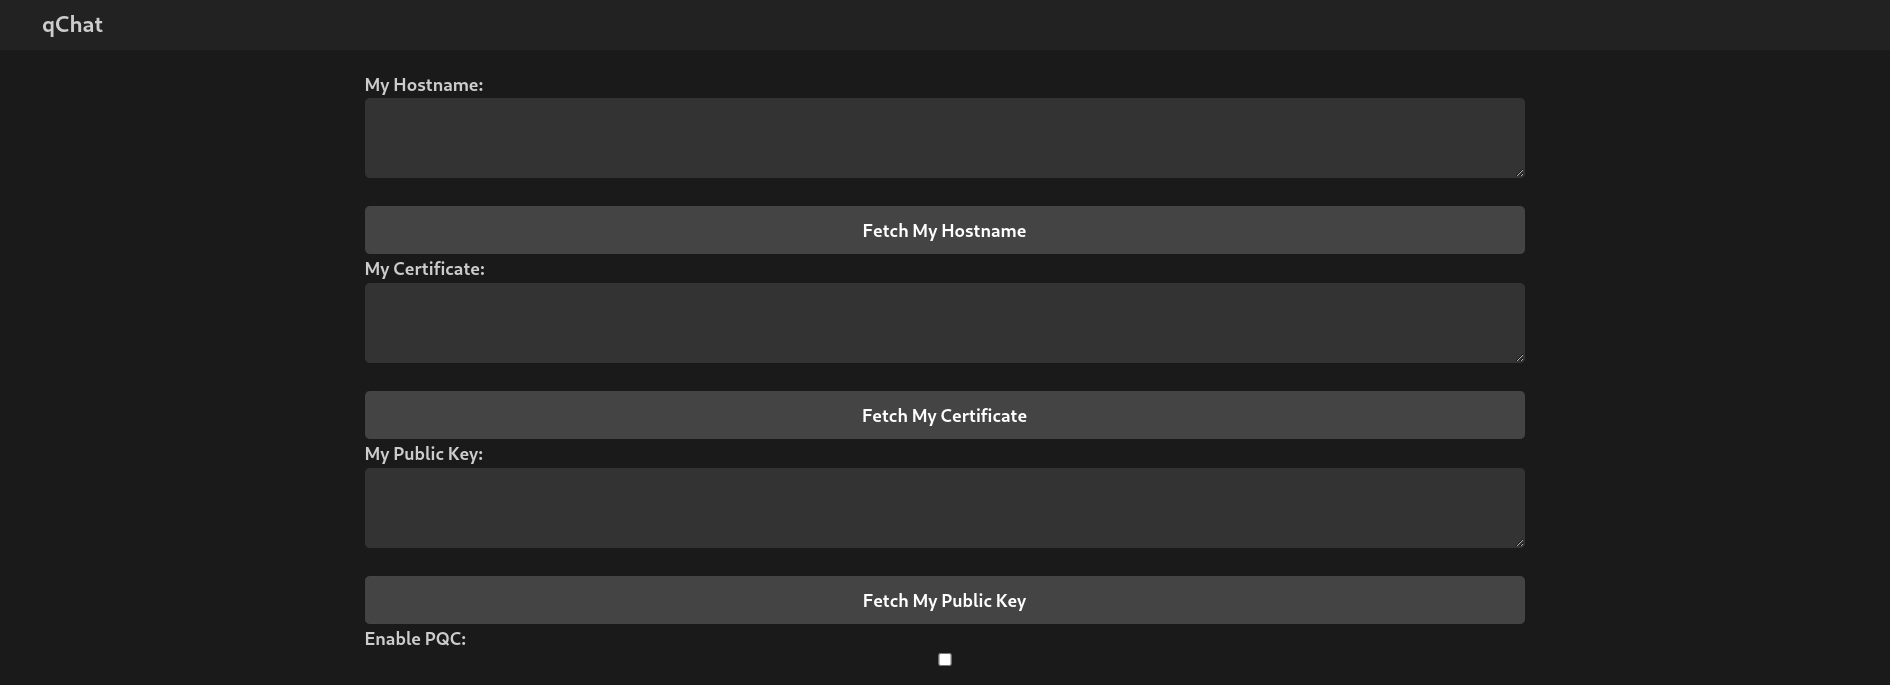
\includegraphics[scale=0.16]{resources/OwnUserCertKey.png}
	\end{center}
\end{frame}

\begin{frame}
	\frametitle{Application - Registration Friend}
	\begin{center}
	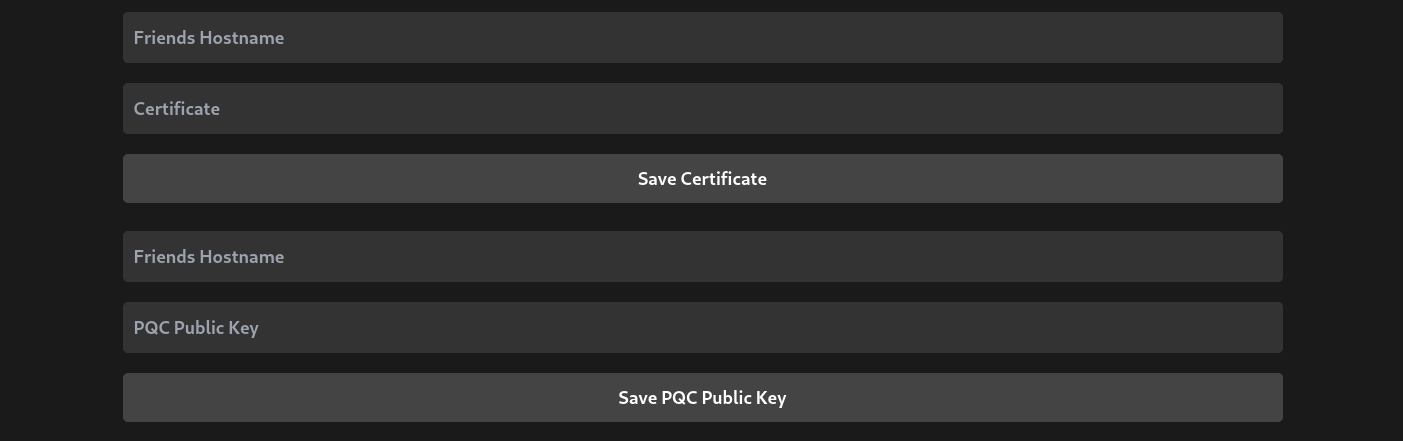
\includegraphics[scale=0.22]{resources/RegistrationFriend.png}
\end{center}
\end{frame}

\begin{frame}
	\frametitle{Application - Send Messages}
	\begin{center}
	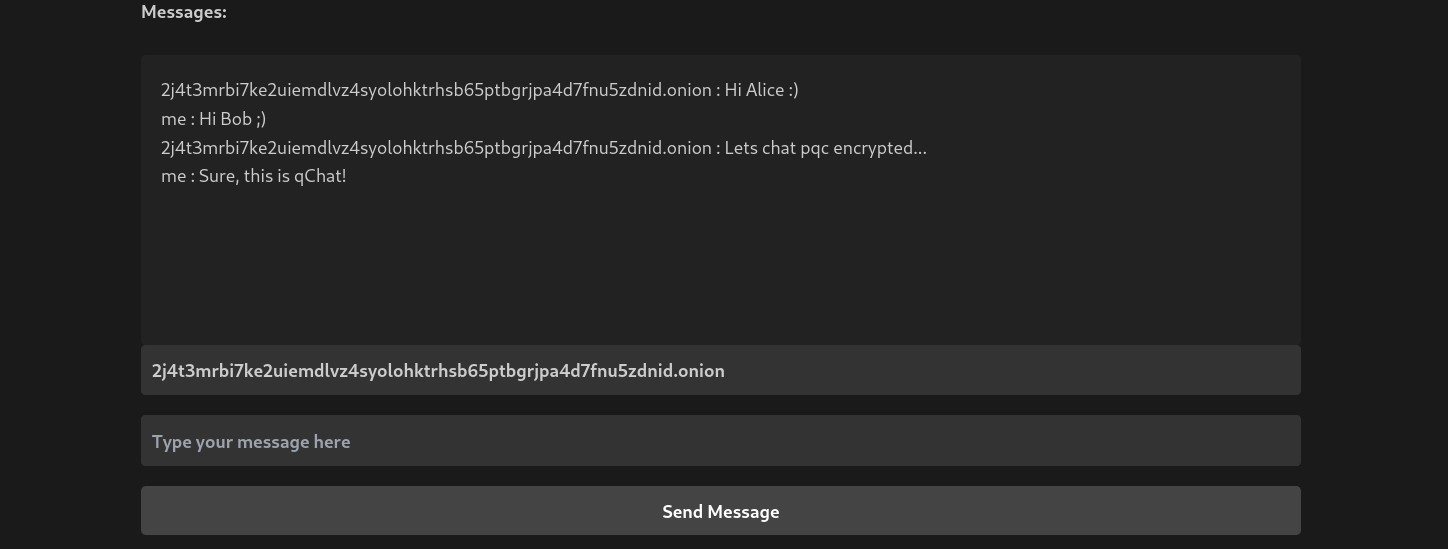
\includegraphics[scale=0.27]{resources/SendMessages.png}
\end{center}
\end{frame}

\begin{frame}
    \frametitle{PQC: Post Quantum Cryptography}
    \vspace{-0.5cm} % Adjust this value as needed
    \begin{center}
        
\includegraphics[scale=0.1]{resources/nist.png}
    \end{center}
    \vspace{-0.5cm} % Adjust this value as needed
    \begin{itemize}
        \item National Institute of Standards and Technology
        \item Round 3 - Crystals-Kyber (KEM)
            \begin{itemize} 
                \item kyber-768 parameter set 
                \item shared library
                \item structured lattices 
            \end{itemize}
    \end{itemize}
\end{frame}


\begin{frame}
	\frametitle{Lattice-based Cryptography}
    \begin{itemize}
        \item BQP (complexity)
        \item LWE Problem (reduction CVP/SVP Problem)
        \item Encapsulates symmetric AES-256 key
        \item Keysize  
        \begin{itemize} 
            \item secret key: 2400 Bytes 
            \item public key: 1184 Bytes
        \end{itemize} 
    \end{itemize}
\end{frame}

\begin{frame}
	\frametitle{CRYSTALS-KYBER}
	\begin{center}
	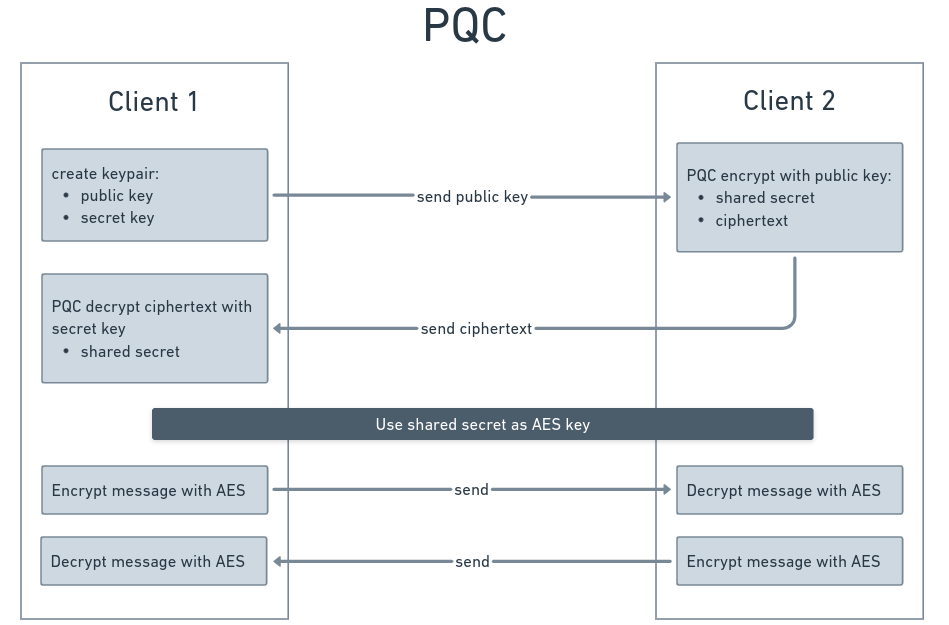
\includegraphics[scale=0.29]{resources/PQC_Diagram.png}
	\end{center}
\end{frame}


\begin{frame}
	\frametitle{Architecture}
	\begin{center}
	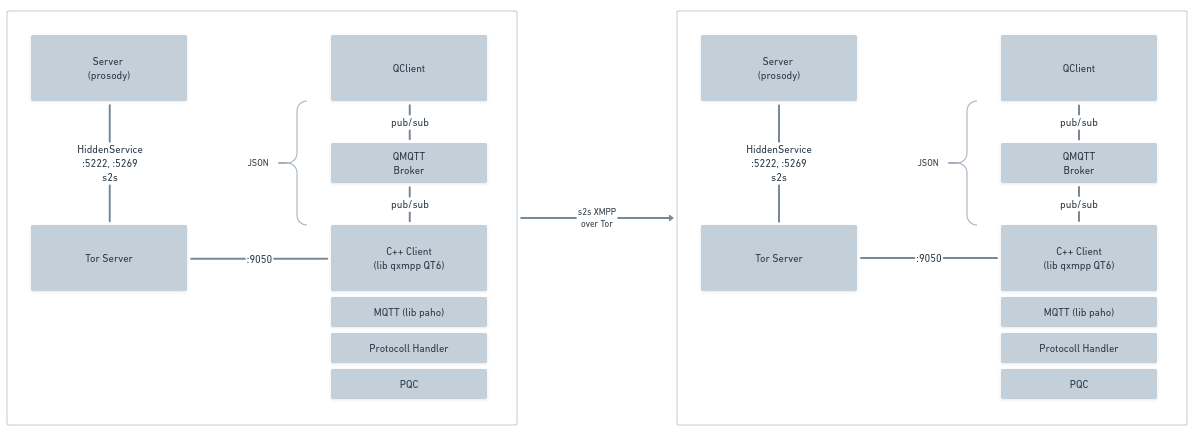
\includegraphics[scale=0.26]{resources/architecture.png}
\end{center}
\end{frame}


\begin{frame}
    \frametitle{ }
    \centering
    \Huge Design Decisions
\end{frame}

\begin{frame}
	\frametitle{Why Tor?}
    \begin{center}
	
\includegraphics[scale=0.05]{resources/tor.png}
    \end{center}
	\begin{itemize}
		\item \textit{Circumvent NAT}
		\item \textit{Anonymity}
		\item \textit{Security (E2E in Tor v3)}
	\end{itemize}
\end{frame}

\begin{frame}
	\frametitle{Why XMPP?}
    \begin{center}
	
\includegraphics[scale=0.05]{resources/xmpp.png}
    \end{center}
	\begin{itemize}
		\item \textit{Well established P2P Protocol}
		\item \textit{Customizable Server Settings (prosody)}
		\item \textit{Lightweight}
		\item \textit{Maintained Libraries for our client (qxmpp)}
		\item \textit{Suited for our client/server design}
	\end{itemize}
\end{frame}

\begin{frame}
	\frametitle{Why MQTT?}
    \begin{center}
	
\includegraphics[scale=0.1]{resources/mqtt.png}
    \end{center}
	\begin{itemize}
		\item \textit{Simple communication between back- and frontend}
		\item \textit{Efficient}
	\end{itemize}
\end{frame}

\begin{frame}
    \frametitle{Security Layers}
    \begin{center}
        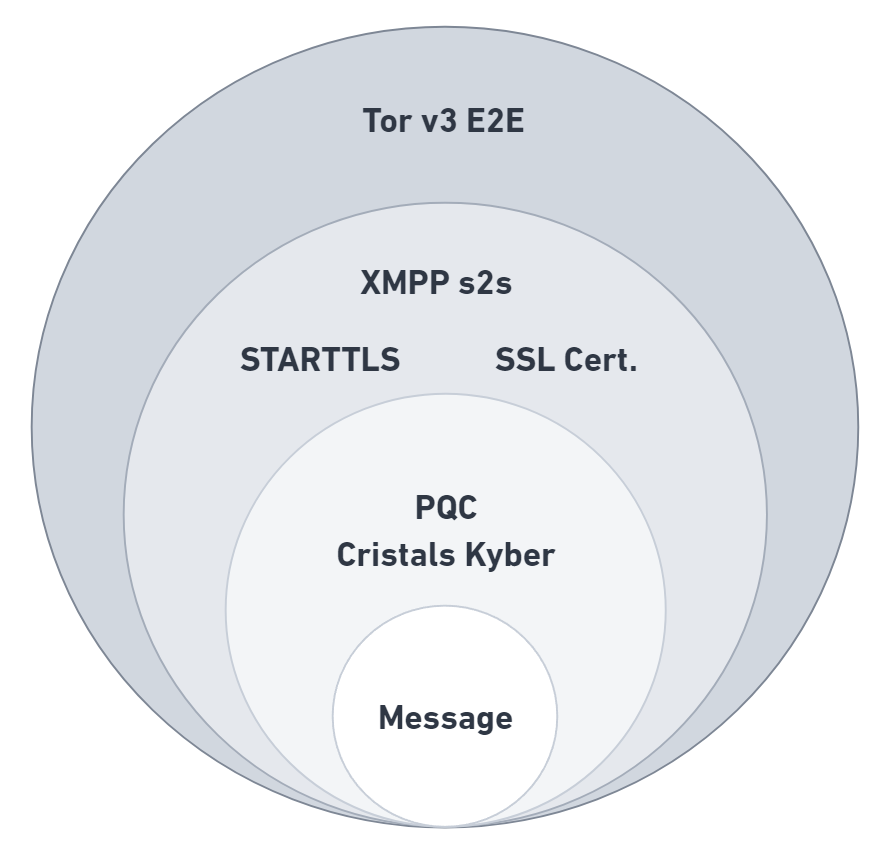
\includegraphics[scale=0.3]{resources/securitylayers.png}
    \end{center}
\end{frame}


\begin{frame}
    \frametitle{ }
    \centering
    \Huge Demo
\end{frame}

\begin{frame}
    \frametitle{ }
    \centering
    \Huge Questions
\end{frame}


\end{document}
